\documentclass[12pt, letterpaper]{article}
\def\blank{\medskip\hrule\medskip}
\usepackage[T2A]{fontenc}
\usepackage[utf8x]{inputenc}
\usepackage[english, russian]{babel}
\usepackage{amsthm}
\usepackage{amssymb}
\usepackage{graphicx} 
\usepackage{wrapfig}
\usepackage{amsmath}
\usepackage[unicode, pdftex]{hyperref}

\renewcommand\qedsymbol{$\blacksquare$}
\renewcommand{\arraystretch}{2} %
\everymath{\displaystyle}

\newtheorem{theorem}{Теорема}[section]
\newtheorem{prop}{Утверждение}[section]
\newtheorem{defi}{Определение}[section]
\newtheorem{sample}{Пример}[section]
\newtheorem{note}{Замечание}[section]

\renewcommand{\O}{\mathbb{O}}
\newcommand{\R}{\mathbb{R}}
\newcommand{\N}{\mathbb{N}}
\renewcommand{\a}{\alpha}
\renewcommand{\b}{\beta}
\renewcommand{\l}{\lambda}
\newcommand{\ph}{\varphi}
\newcommand{\e}{\varepsilon}
\newcommand{\leqp}{\leq_{p}}
\newcommand{\leql}{\leq_{l}}

\usepackage[%
    left=0.50in,%
    right=0.50in,%
    top=0.50in,%
    bottom=0.50in,%
    paperheight=11in,%
    paperwidth=8.5in%
]{geometry}%

\begin{document}

\section{Билет 1}
\begin{prop}
Пусть $M$ -- одноленточная МТ, которая распознает язык бинарных палиндромов. Тогда существует константа $C : \exists n_o : \forall n > n_0$ существует вход длины $n$, на котором $M(x)$ делает $\geq Cn^2$ шагов.
\end{prop}

\begin{proof}
В начале очевиден принцип несжимаемости, нельзя инъективно перевести строки из $\{0, 1 \}^n$ в $\{0, 1\}^*$ так, чтобы все образы по длине были меньше чем $n$.\\
Будем доказывать для входов, длина которых кратна 3. По $x \in \{0, 1\}^n$ строим вход $x 0^n x^{rev}$ и скармливаем МТ все такие входы. Возьмем все перегородки после нулей, их всего $n$, существует перегородку, через которую МТ прошла $\leq \frac{T(x)}{n}$ раз. \\
Теперь строим отображение $f : \{0, 1\}^n \rightarrow \{0, 1\}^{*}$, переводим строку $x$ в протокол работы МТ на строке $x 0^n rev(x)$. Для этого выпишем набор состояний, в которые переодила МТ, переходя через "хорошую" перегородку и номер этой перегородки. \\
Утверждается, что такая $f$ -- инъекция, чтобы доказать, предположите обратное и рассмотрите работу на строке $x0^n y^{rev}$.\\
Пусть $|x|=n$, тогда $f(x) \leq \log n + \frac{T(x)}{n} C$, но при этом существует $|y|=n$, такой что $f(y) \geq n$. Получаем, что 
$$n \leq log n + \frac{T(x)}{n} C $$
$T(x) = \omega(n^2) $ на таких входах. \\
Для некратных 3 входов делаем также, но по-середине пишем вместо $n$ нулей, на один ноль больше или меньше -- это не влияет на оценки.
\end{proof}

\section{Билет 2}
\begin{defi}
$k$ -- ленточная машина Тьюринга. (Добавляется куча лент и функция перехода теперь действует по всем лентам).
\end{defi}

\begin{prop}
Для любой $k$ -- ленточной МТ, которая на входе $x$ работает время $T(x)$, существует 1 ленточная МТ, которая работает $O(T(x)^2)$.
\end{prop}
\begin{proof}
Будем хранить в одном символе МТ символы всех лент (а также спец символы, помеченные головкой). На каждом шаге будем идти вправо и делать все изменения, которые нужны на лентах. 
\end{proof}

\begin{defi}
Универсальная МТ -- эмулирует МТ по описанию.
\end{defi}

\begin{prop}
Для любой $k$-ленточной МТ существует универсальная $k$-ленточная МТ с линейным замедлением.
\end{prop}
\begin{proof}
Понятно как получить квадратичное замедление, нужно положить описание в начало, например, первой ленты. Далее постоянно возвращаться, чтобы узнать, какой шаг сделать. Если же хотим линейного -- давайте возить описание с собой, это будет давать $O(1)$ действий из-за его константного размера, при этом эмуляция будет работать за линейное время.
\end{proof}

\begin{prop}
$k$ ленточную МТ можно эмулировать на 2-ленточной с логарифмическим замедлением.
\end{prop}
\begin{proof}
TODO
\end{proof}


\section{Билет 3}
Основная модель вычислений -- многоленточная МТ. 
\begin{defi}
$f : \mathbb{N} \rightarrow R_{+}$, тогда $L \in DTime[f(n)]$, если 
существует многоленточная МТ, такая что
\begin{enumerate}
\item $\forall x \in L \Rightarrow M(x) = 1$.
\item $\forall x \notin L \Rightarrow M(x) = 0$.
\item $\forall x$ МТ работает $O(f(|x|)$ шагов.
\end{enumerate} 
\end{defi} 

\begin{defi}
$P = \cup_{i>0} DTime[n^i]$.
\end{defi}

\begin{defi}
Про семейство схем, распознающих язык.
\end{defi}

\begin{defi}
$L \in Size[f(n)]$, если есть последовательность схем, распознающих L и для достаточно больших $n$ выполнено $|C_n| \leq f(n)$.
\end{defi}

\begin{defi}
$P/Poly = \cup_{i>0} Size[n^i]$.
\end{defi}

\begin{sample}
Неразрешимый язык может лежат в $P/Poly$. Например $1^{H}=\{1^{n} | n \in H \}$, для некоторого языка тоже является разрешимым и лежит в $P/Poly$, так как на каждую длину мы можем предоставить схему.  
\end{sample}

\begin{prop}
Существует такой алгоритм $A$, который получает на вход $T,n,m$ и 
\begin{enumerate}
\item $A$ работает $poly(n + T + |m|)$ шагов.
\item Если МТ $m$ на всех входах из $\{0,1\}^{*}$ выдает ответ за $\leq T$ шагов, то алгоритм $A$ выдает схему $C$, которая имеет $n$ входов и 1 выход и распознает на входах длины $n$ также как $m$.
\end{enumerate}
\end{prop}
\begin{proof}
Будем возвращать схему размера $T \times T \cdot O(1)$.\\
На уровне $i$ будет $T$ ячеек, в каждой из которых будет вычисляться некоторая информация: сивмол, написанный в этой ячейке, есть ли тут головка в момент $i$, а также, если есть головка, то состояние, в которой МТ сейчас находится. Понятно, что для пересчета этих параметров нужно обратиться к нескольким соседним ячейкам предыдущей строки. Для того, чтобы узнать ответ, посмотрим, принималось ли где-нибудь состояние $q_{yes}$.\\
\end{proof}

\begin{prop}
$P \subseteq P/Poly$.
\end{prop}

\begin{note}
Таким образом хотели доказывать, что $P \neq NP$, взять, к примеру, $SAT$ и показать, что он не лежит в $P / Poly$, однако доказывать нижние оценки на схемы пока что не научились.
\end{note}

\section{Билет 4}
\begin{defi}
$L \subseteq \Sigma^{*}$, система доказательств для языка $L$ -- это такой алгоритм $\Pi$, который обладает следующими свойствами:
\begin{enumerate}
\item (Полнота) $\forall x \in L \Rightarrow \exists w : \Pi(x,w)=1$
\item (Корректность) $\forall x \notin L \Rightarrow \forall w \Pi(x,w) \neq 1$ 
(Ну или равно 0).
\item $\Pi$ всегда останавливается  
\end{enumerate}
\end{defi}

\begin{defi}
Система доказательств $\Pi$ называется эффективной, если $\Pi(x,w)$ работает за $\leq poly(|x|+|w|)$ шагов.
\end{defi}

\begin{note}
Системы доказательств существуют для перечислимых языков, как мы знаем из предыдущий главы курса. Также можно доказать, что для всех перечислимых языков существует и эффективная система доказательств ($TCS12$), искуственно увеличивая подсказку.
\end{note}

\begin{defi}
класс $NP$ состоит языков, для которых существует эффективная система доказательств $\Pi$, а также полином $q$, такой что $\forall x \in L \exists w, |w| \leq q(|x|), \Pi(x,w)=1$, то есть, существует полиномиальная подсказка.
\end{defi}

\begin{sample}
Примеры языков из $NP$.
\begin{enumerate}
\item $SAT$ -- множество выполнимых пропозициональных формул. \\
$SAT \in NP$, но не выяснено, $UNSAT \notin/\in NP$.
\item $Hampath$ -- язык графов, в которых есть гамильтонов путь, также лежит в $NP$.
\item $CLIQUE$ -- язык пар (граф, число) такой, что в графе есть клина на числе вершин. Лежит в $NP$.
\item $Composite$ -- язык составных натуральных чисел, лежит в $NP$, а также, известно, что $Primes \in NP$ ($TCS11$) и, более того, человечество умеет показывать $Primes \in P$.  
\end{enumerate}
\end{sample}

\begin{defi}
Недетерминированные МТ. Вместо одной функции перехода теперь две и машина сама выбирает, в какую идти. ($:)$).\\
Говорят, что недетерминированная $M$ принимает слово, если существует последовательность корректных переходов, при которых она придет в состояние $q_{yes}$ на входе этом слове. \\
Время работы НМ -- максимум по всем возможным применениям функции перехода.
\end{defi}

\begin{defi}
$NTime[f(n)]$ -- множество языков, которые принимаются многоленточными НМТ за $O(f(n))$ шагов, где $n$ -- длина входа.
\end{defi}

\begin{defi}[Второе определение $NP$]
$NP = \cup_{c>0} NTime[n^c]$.
\end{defi}

\begin{defi}[МТ с подсказкой].
К обычной МТ добавляется лента подсказки, на которую записывается некоторая строка, к которой может обращаться МТ во время работы. Машина принимает слово, если существует подсказка, для которой она придет в состояние $q_{yes}$. Время работы такой машины -- максимум по всем подсказкам.
\end{defi}

\begin{theorem}
Следующие условия эквивалентны:
\begin{enumerate}
\item $L \in NP$ (на языке систем доказательств)
\item $L$ распознается машиной Тьюринга с подсказкой за полиномиальное время.
\item $L \in \cup_{c>0} Ntime[n^c]$.
\end{enumerate}
\end{theorem}

\begin{proof}
$(1) \Rightarrow (2)$: построим МТ с подсказкой. Пусть наша МТ при обращениях к подсказке будет теперь обращаться на ленту с подсказкой вместо ленты входа. Тогда понятно, что подсказки аналогичны друг другу.\\
$(2) \Rightarrow (3):$ пусть МТ порождает подсказку, а далее действует детерминированно. Подсказка более чем полиномилаьного размера не нужна, так как наш алгоритм не успеет ее обработать из-за своего времени работы.\\
$(3) \Rightarrow (1):$ подсказка -- какую функцию перехода выбирать на каждом шагу. 
\end{proof}

\section{Билет 5}
\begin{defi}
Язык $A$ сводится по Карпу к языку $B$, если существует полиномиально вычислимая $f$: $\forall x, x \in A \Longleftrightarrow f(x) \in B$. Обозначается $A \leq_{p} B$.
\end{defi}
\begin{prop} Свойства сведения
\begin{enumerate}
\item $A \leqp B$, $B \in P \Rightarrow A \in P$.
\item $A \leqp B, B \leqp C \Rightarrow A \leqp C$. 
\end{enumerate}
\end{prop}

\begin{defi}
Язык $A$ называется $NP$-трудным, если $\forall L \in NP, L \leqp A$. Язык A $NP$-полный, если $A\in NP$ и $A$ -- $NP$-трудный. 
\end{defi}

\begin{defi}
$BH = \{ (M, x, 1^t) | $ $\exists y, M(x,y)$ выдает 1 за $\leq t$ шагов  $\}$. 
\end{defi}

\begin{theorem}
$BH$ -- $NP$-полный.
\end{theorem}
\begin{proof}
Проверим, что $BH \in NP$. Подсказка как раз и будет этот $y$. Запускаем на $t$ шагов и проверяем, приняло или нет. Если тройка лежит в языке, то по определению найдется такая подсказка, что выдаст $yes$. Иначе -- нет.\\
Возьмем $L \in NP$, хотим проверить $L \leqp BH$. У $L$ есть нмт эффективная система доказательств $\Pi$, работающая за $q(|x|+|y|)$, при этом также для лежащих в языке слов есть маленькая подсказка, длины $\leq p(x)$. Давайте сделаем следующее отображение $f(x) = (M, x, 1^{q(|x|+p(|x|))})$. Очевидно, что это корректное сведение.

\end{proof}

\section{Билет 6}
\section{Билет 7}

\section{Билет 8}
\begin{theorem}[Ладнер]
Если $P \neq NP$, то существует $L \in NP$, такой, что, $L \notin P$ и $L$ -- не полный в $NP$.
\end{theorem}
\begin{proof}
Интуиция следующая: хотим немного ослабить язык $SAT$. Давайте рассматривать 
$$SAT_H = \{\ph 0 1^{n^{H(n)}} | \ph \in SAT, |\ph| = n \} $$
Поймем, как определить $H$. 
Возьмем нумерацию всех машин Тьюринга $M_1, M_2, M_3, \ldots$.\\
$H(n) = i$, если $i$ -- такое минимальное число, что $i < \lfloor \log \log n \rfloor$, что $M_i$ решает $SAT_H$ на всех входах $|x| \leq \log n$ за время $i|x|^i$, или, если такого числа нет, то $\lfloor \log \log n \rfloor$.\\
Заметим, что $H(n)$ определяется через $SAT_H$ и наоборот. \\
Но заметим, что чтобы определить $H(n)$ нам не потребуется значений $H(x)$ при $x > \log n$, так как $H(n)$ нужно для дописывания только к строкам длины $n+1$. 

\begin{prop}
$H(n)$ вычисляется по значениям $H(1), \ldots, H(n-1)$ за $poly(n)$ действий. 
\end{prop}
Будем вычислять по определению. Переберем \begin{enumerate}
\item $i \leq \log \log n$
\item $x, |x| \leq \log n$, это $2^{\log n} = O(n)$ действий
\item запустим машину $i$ на $(\log \log i) (\log i)^{\log \log i} = $ действий.
\item Сравним результат с реальным: мы можем понять, лежит или нет, так как знаем предыдущие значения $H$, $SAT$ будем решать перебором за $O(n)$.	
\end{enumerate}
Таким образом вычислим $H(n)$ за $O(n^3)$ по предыдущим значениям. Тогда мы сможем вычислить $H(n)$ за $O(n^4)$, вычисляя по очереди все значения.

\begin{prop}
$H(n)$ не убывает.
\end{prop}
Действительно, если $H(n)=i$, то такое $i$ подошло и для всех предыдущих, либо $i$ -- верхняя граница для $H(n)$, но тогда оно точно больше предыдущих.

\begin{prop}
$SAT_H \in P \Longleftrightarrow H(n) \leq C$.
\end{prop}
$\Rightarrow:$ есть МТ, решающая $SAT_H$ за $p(|x|)$. Но эта МТ встречается в нумерации бесконечное число раз. Она там также встречается как $M_i$ при $i|x|^i > p(|x|)$. Но тогда $H(n) \leq i$, так как такая машина нам все решит и мы ее запустим на такое число шагов.\\
$\Leftarrow:$ Ограниченная неубывающая функция это такая функция, что с некоторого момента она равна $j$. Но заметим, что тогда $M_j$ решит нам язык за $j|x|^j$, что есть полином.
\end{proof}

\begin{prop}
$SAT_H \in NP$
\end{prop}
Действительно, давайте просто давать как подсказку решение для внутренней $SAT$, при этом определить, верное ли кол-во единиц мы можем, вычислив $H$.

\begin{prop}
$SAT_H \notin P$. 
\end{prop}
Пусть это не так. Тогда $H(n)$ ограничена. Тогда $SAT \leqp SAT_H$ и $P=NP$.

\begin{prop}
$SAT$ не сводится к $SAT_H$ полиномиально.
\end{prop}
Предположим обратное. Покажем тогда, что мы сможем решить $SAT$ за полином. Пусть сведение работает за $n^c$. Тогда величина формулы, которую выдаст сведение $\leq n^c$, где $n$ -- длины формулы, поступившей нам на вход. \\
$H(n)$ не ограничена, возьмем $n_0$ такое, что $H(n) > 3c$ при $n > n_0$. Тогда пусть сведение выдало битовую строку, длина которой $m > n_0$ (иначе сделаем полный перебор, который займет $O(1)$) и у которой правильное число единиц на конце (иначе мы это легко проверим за полином).\\
Тогда $m \geq |\ph| + 1 + |\ph|^{3c}$, отсюда $|\ph| \leq m^{1/3c}$, при этом $m \leq n^c$. Получается, $|\ph| \leq n^{1/3}$. При больших $n$ такое значение хотя бы в 2 раза меньше $n$. Значит, мы свелись к формуле меньшего размера в 2 раза. Таким образом мы сделаем не более $\log$ полиномиальных сведений и выдадим верный ответ. Отсюда $P = NP$ и противоречие.

\section{Билет 9}
\begin{sample}
$DTime[n^2]\subsetneq DTime[n^3]$.
\end{sample}
\begin{proof}
Давайте диагонализировать.                 
$$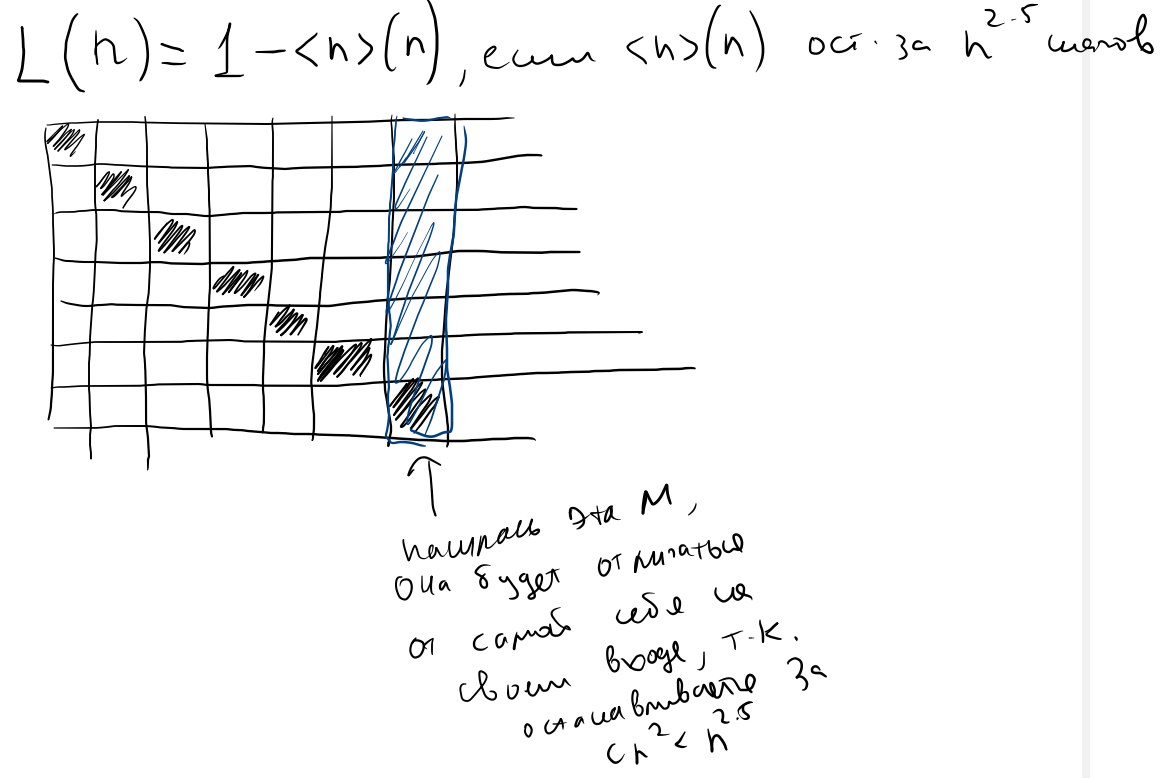
\includegraphics[scale=0.6]{diag.png}$$  
Рассмотрим язык $L = \{M | M$ отвергает $M$ за не более $|M|^{2.5}$  $\}$.
Пусть он решается квадратичной $M$ за $Cn^2$ шагов. Тогда давайте найдем эквивалентную ей $M'$ такую, что $|M'|^{2.5} > C|M'|^2$. Тогда получится, что $M'$ не равна себе же в строчке, соответствующей $M'$. \\
Как показать, что $L \in DTime[n^3]$? Давайте эмулировать МТ, которая работает $O(n^{2.5})$ с логарифмической задержкой.\\
Тогда получили нужный язык $L$. 
\end{proof}

\begin{defi}
$h : \N \rightarrow \N$ -- конструктивная по времени, если $n \rightarrow h(n)$ можно вычислить за $O(h(n))$ шагов на ДМТ.
\end{defi}

\begin{theorem}[Об иерархии по времени для детерменированных вычислений]
$f,g,h : \N \rightarrow \N$, $h$ -- конструктивная по времени.\\
$f(n) = o(h(n)), h(n)\log h(n) = o(g(n))$, тогда $DTime[f(n)] \subsetneq Dtime[g(n)]$.
\end{theorem}

\begin{proof}
Конструкция такая же, как и в предыдущем утверждении. Конструктивная функция нужна для будильника в МТ. $\log$ -- для эмуляции.
\end{proof}

\begin{prop}
$P \subsetneq EXP$.
\end{prop}
\begin{proof}
$P \subseteq DTime[2^n] \subsetneq DTime[2^{n^2}] \subseteq EXP$.
\end{proof}

\begin{note}
Доказательство не работает для НМТ, потому что мы не можем реверснуть ответ за такое же время.
\end{note}

\begin{sample}
$NTime[n^2] \subsetneq NTime[n^3]$.
\end{sample}
\begin{proof}
Определим для $M_i$ из перечисления всех НМТ отрезок $[n_i, n_i^{*}]$ так, что $n_i^{*} = 2^{n_i^{2.5}}$. \\
$n_{i+1} = n_i^{*}+1$.\\
$[n_1, n_1^{*}], [n_2, n_2^{*}], [n_3, n_3^{*}], \ldots$.\\
Определим язык $L$ так:
\begin{enumerate}
\item $L(n_i^{*}) = 1 - M_i(0^{n_i})$, если $M_i(0^{n_i})$ завершилось за менее чем $n_i^{2.5}$ шагов и 0 иначе.
\item $L(n) = M_i(0^{n+1})$ для $n_i \leq n < n_i^{*}$ 
\end{enumerate}
\begin{prop}
$L \notin NTime[n^2]$.
\end{prop}
Пусть это не так, тогда есть $M$, решающая $L$ за $Cn^2$. Возьмем такое ее вхождение, что $\forall n \in [n_i, n_i^{*}], n^{2.5} > Cn^2$. Тогда:
$$M(0^{n_i}) = L(0^{n_i}) = M(0^{n_i+1}) = L(0^{n_i+1}) = \ldots = L(0^{n_i^{*}}) \neq M(0^{n_i}) $$
так как все машины успеют отработать.
\begin{prop}
$L \in NTime[n^3]$. Разбираем случаи, если надо проэмулировать, то эмулируем, иначе нам нужно реверснуть выход недетерменированной машины. Мы можем сделать это за $2^{n_i^{2.5}} \cdot n_i^{2.5} < ((n_i)^{*})^3$.
\end{prop}
\end{proof}

\begin{theorem}[Об иерархии по времени для недетерменированных вычислений].
$f,g,h : \N \rightarrow \N$, $h$ -- конструктивная по времени.
$f(n) = o(h(n))$, $h(n+1) = o(g(n))$, тогда $NTime[f(n)] \subsetneq NTime[g(n)]$.

\begin{prop}
$NP \notin NEXP$.
\end{prop}
\begin{proof} аналогично детерменированному случаю.\end{proof}

\end{theorem}

\section{Билет 10}	
\begin{defi}[Модель вычислений с ограничением по памяти.]
 МТ с дополнительной лентой входа, она read-only, также по ней нельзя уйти правее первого пробела. Также есть лента выхода, по которой нельзя двигаться влево, а только выдавать очередной символ ответа. Затраченная память -- максимальный уход вправо на какой-то из рабочих лент.
\end{defi}

\begin{defi}
$DSpace[f(n)]$ -- класс языков, которые принимают ДМТ, использующие $O(f(n))$ памяти. $NSpace[f(n)]$ -- то же самое, но для НМТ.
\end{defi}

\begin{defi}
$PSPACE = \cup_{c>0} DTime[n^c]$, $NPSPACE = \cup_{c>0} NTime[n^c]$.
\end{defi}

\begin{defi}
$L = LOGSPACE = DSPACE[\log(n)]$, $NL = NSPACE[\log n]$.
\end{defi}

\begin{prop}
$\forall s(n)$ : $DTime[s(n)] \subseteq DSpace[s(n)] \subseteq NSpace[s(n)]$.
Причем первое включение работает лишь для некоторых моделей вычислений. В частности, для МТ.
\end{prop}

\begin{defi}
$S : \N \rightarrow \N$ -- конструктивная по памяти, если $1^{S(n)}$ можно вывести за $O(S(n))$ памяти.
\end{defi}

\begin{theorem}
$s(n)$ -- конструктивная по памяти и $s(n) \geq \log n$. Тогда 
$$NSpace[s(n)] \subseteq DTime[2^{O(s(n)}] = \cup_{c>0} DTime[2^{cs(n)}]$$.
\end{theorem}
\begin{proof}
Для доказательства используется идея с графом конфигураций. Конфигурация МТ это набор параметров:
\begin{enumerate}
\item Положение головок на всех лентах
\item Содержание рабочих лент
\item Состояние
\end{enumerate}
Проблема выяснения того, принимает ли МТ вход $x$ может быть рассмотрена как проблема выяснения существования пути в графе конфигураций.  
 Поймем, сколько есть конфигураций:\\
$n \cdot (C s(n))^k$ -- положение головок, $2^{c' s(n) k}$ -- содержимое рабочих лент. Если $s(n) \geq \log n$, то это число есть $2^{O(s(n))}$. В таком случае мы можем сгенерировать такой граф и проверять наличие пути полиномиальным алгоритмом. Получится время работы $poly(2^{O(s(n))} = 2^{O(s(n))}$. \\
Зачем пользовались конструктивностью функции по времени? Для того чтобы сгенерировать конфигурацию нужно отмерить максимальную длину конфигурации и дальше уже перебирать все возможные строчки. Поэтому хочется уметь отмерить за нормальную память. \\
То есть итоговый алгоиртм такой: по $M, x$ строим граф конфигураций и ищем путь из $K_0$ в $K_{accept}$. Можно сделать одно состояние $K_{accept}$, попросив МТ стирать все рабочие ленты перед тем как завершиться. Так мы унифицируем конечные состояние, но, очевидно, не изменим вычислительную мощь ($:)$).
\end{proof}

\begin{prop}.
\begin{enumerate}
\item $NSPACE \subseteq EXP$
\item $NP \subseteq EXP$  
\end{enumerate}
\end{prop}

\begin{theorem}[Савич]
$s(n)$ -- конструктивная по времени и $s(n) \geq \log n$, тогда $NSpace[s(n)] \subset DSpace[s(n)^2]$.
\end{theorem}
\begin{proof}
Все сводится к тому, чтобы по графу понять, есть ли в нем путь от вершины до другой за память $s(n)^2$, где $s(n)$ -- память рассматриваемой НМТ. Воспользуемся предикатом $PATH(u,v,i)$ -- есть ли путь от $u$ до $v$ длины не более $2^{i}$ и рекурсивным перебором. 
\end{proof}

\begin{prop}
$NPSPACE = PSPACE$
\end{prop}
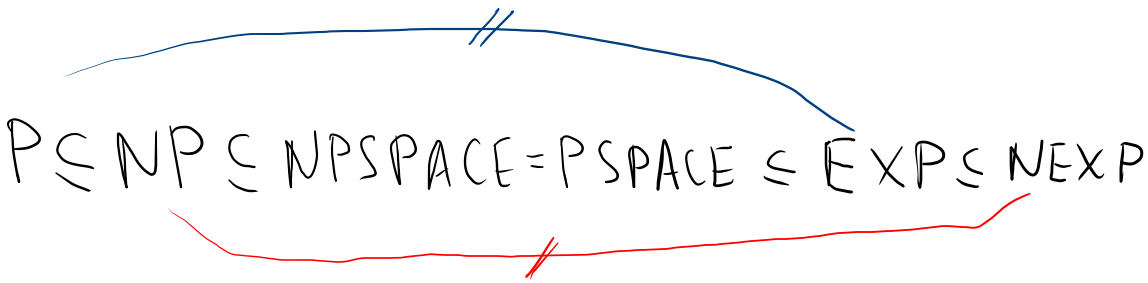
\includegraphics[scale=0.6]{hierarchy1.png}

\section{Билет 11}
Рассмотрим кванторные пропозициональные формулы: $Q_1 x_1, \ldots, Q_n x_n \ph(x_1, \ldots, x_n)$. Язык таких истинных формул это $TQBF$. Понятно, что $SAT \leqp TQBF$ просто дописываниям ко всем переменным квантора существования.\\
\begin{prop}
$TQBF$ лежит в $PSPACE$ 
\end{prop}
Действительно, можно просто сделать перебор рекурсивно и проверить выполнимость.

\begin{prop}
$TQBF$ -- полный в классе $PSPACE$.
\end{prop}
\begin{proof}
Берем граф конфигураций. Хотим записать формулу $PATH(K_0, K_{accept}, cp(n))$. (время работы не более $2^{cp(n)}$, так как иначе все зациклится).\\
Будем записывать при помощи следующего выражения: \\
$PATH(u, v, i) = \exists z \forall A, B ((A=u, B=z) \vee (A=z, B=v)) \rightarrow PATH(A, B, i-1)$, тогда мы сможем записать всё за полиномиальное количество бит. Остаются детали, как записать в виде формулы утверждения вида $PATH(u, v, 0)$. Мы можем с помощью полиномиального алгоритма проверить такой предикат. \\
Еще нужно подумать о том, как записать равенство конфигураций, это можно сделать просто побитово.
\end{proof}

\begin{note}
Выяснение вопроса детерменированной победы в конечных играх -- задача из $PSPACE$, так как ее можно записать в $TQBF$ в виде $\exists step_{1,1} \forall step_{2,1} \exists step_{1,2} \ldots Q(..)$, что означает, что есть ход первого игрока, что при любом ходе второго есть ход первого и тд, что первый игрок выиграл.
\end{note}

\section{Билет 12}
\begin{defi}[Логарифмическое сведение]
$A \leql B$, если существует $p$, вычислимая с использованием логарифмической памяти такая что $x \in A \Longleftrightarrow p(x) \in B$.
\end{defi}

\begin{prop}[Свойства лог сведений]
\begin{enumerate}
\item $A \leql B \Rightarrow A \leqp B$.
\item $A \leql B, B \leql C \Rightarrow A \leql C$.
\item $A \leql B, B \in L \Rightarrow A \in L$.
\end{enumerate}
\end{prop}
Чтобы доказать эти утверждения нужна лемма.
\begin{prop}
$f, g$ -- вычислимые с логарифмической памятью. Тогда $f \circ g$ тоже вычислима с логарифмической памятью. 
\end{prop}
\begin{proof}
Будем вычислять $f(g(x))$, когда для вычисления $f$ будет требоваться очередной бит входа, будем вычислять $i$-тый бит выхода $g(x)$ заново и ждать пока выведется бит под номером $i$. 
\end{proof}
$L \in NL$, а вот есть ли равенство -- открытый вопрос.
\begin{defi}[Определение NL через систему доказательств]
У нас появляется лента для подсказки, по которой можно двигаться только вправо (потому что НМТ не может записывать результат выбора на ленту). Это задает такой же класс языков, это можно видеть также как мы видели для разных определений $NP$.
\end{defi}
\begin{defi}
$DPATH = \{(G, u, v) |$ в ор. графе $G$ есть путь $u \rightarrow v$ $\}$. 
\end{defi}
$DPATH \in NL$, подсказкой является собственно путь. Нужно проверить, что первая вершина в нем есть $u$, последняя $v$ и что есть ребро между соседними, это можно сделать за $\log$ памяти.

\begin{theorem}
$DPATH$ -- $NL$ полный (относительно $\leql$).
\end{theorem}
\begin{proof}
пусть $A \in NL$, $M$ -- нмт, решающая $A$. Сведение будет следующим. Оно будет генерировать конфигурации, которые составляют максимум $\log$ памяти и выводить ребра между ними, то есть строить граф конфигураций. Далее выведем начальное и конечное состояние и это и будет искомый инстанс задачи $DPATH$.
\end{proof}

\begin{note}
Неизвестно, лежит ли $DPATH$ в $L$, или нет.
\end{note}

\begin{theorem}
$\overline{DPATH} \in NL$
\end{theorem}

\begin{proof}
Нам нужно сертифицировать, что между $s, t$ нет пути, причем сделать такое доказательство, которое можно читать слева направо и использовать логарифмическую память. \\
$U_i$ -- множество вершин, до которых есть путь от $s$ длины не более $i$. \\  
\begin{enumerate}
\item для $v$ можно сертифицировать, что $v \in U_i$, сертификат -- просто путь, как в языке $DPATH$.
\item если известно $|U_{i-1}|=k$, то можно сертифицировать, что $u \notin U_i$. Для этого предоставим список вершин из $U_{i-1}$ с сертификатами, что они действительно оттуда. Причем список будет у нас возрастающим, чтобы не было повторяющихся вершин. Проверим, что там правильное число вершин + нет вершины $u$ и также нет ребра между вершинами из списка и $u$. 
\item если известно $|U_{i-1}|=k$, то можно сертифицировать, что $|U_i| = t$. Просто для каждой вершины напишем одно из двух, либо сертификат того, что она лежит в $U_{i}$, либо сертификат того, что не лежит, при условии $|U_{i-1}|=k$.
\item Таким образом мы можем сертифицировать, что размер $U_{n-1}=k$ и что $t \notin U_n$. 
\end{enumerate}
\end{proof}

\begin{defi}[coЯзык]
$X$ -- класс языков. Тогда $coX = \{ \Sigma^* \setminus L | L \in X \}$. 
\end{defi}

\begin{note}
Как мы уже видели, $NP = coNP$ -- неизвестно.
\end{note}

\begin{theorem}
$s(n) \geq \log n$ -- конструктивная по памяти. Тогда $NSpace[s(n)]=coNSpace[s(n)]$.
\end{theorem}
\begin{proof}
$A \in NSPACE[s(n)]$, хотим показать, что $A \in coNSpace[s(n)] \Longleftrightarrow \overline{A} \in NSpace[s(n)] $. Причем, если покажем это, то автоматически последует равенство, так как для $A \in coNSpace[s(n)]$ надо показать, что $\overline{A} \in Nspace[s(n)]$, тогда из той стрелочки, которая описана это последует.\\
Рассмотрим $M$ -- НМТ, которая распознает $A$ с памятью $cS(n)$. $x \in \overline{A} \Longleftrightarrow x \notin A \Longleftrightarrow$ в графе конфигураций $G_x$ из $K_0$ нет пути в $K_{accept}$.\\
Сертификатом будет тот же самый, сертификат, что и был в теореме выше. Размер графа конфигураций будет $2^{O(s(n))}$, тогда нам потребуется $O(s(n))$ памяти, чтобы проверить сертификат. Причем граф строить полностью не надо, нужно всего лишь уметь проверять, есть ли некоторые ребра в нем. 
\end{proof}
\begin{note}
Выяснили на нынешний момент следующую картинку:\\
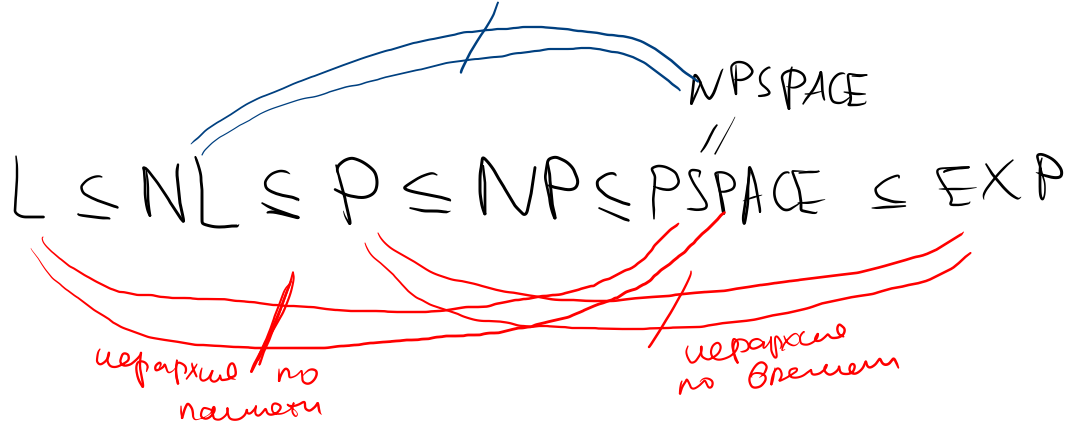
\includegraphics[scale=0.5]{hierarchy2.png}
\end{note}

\section{Билет 13}
\begin{defi}
Определение классов $\Sigma^P_0, \Sigma^P_1, \ldots$, а также $\Pi^P_0, Pi^P_1$.
\end{defi}
Интуиция про $NP, coNP$ и $\Sigma^P_1, \Pi^P_1$.\\
Можно развернуть определение:
$\forall x, x \in L \Longleftrightarrow \exists y_1 |y_1| \leq p(|x|) \forall y_2 , \ldots, y_i Q(x_, y_1, \ldots, y_i)$.
\begin{defi}
$PH = \cup_{i\geq0} \Sigma^P_i$
\end{defi}
\begin{prop}[Свойства полиномиальной иерархии].
\begin{enumerate}
\item $\Sigma^P_i \cup \Pi^P_i \subseteq Sigma^P_{i+1} \cap Pi^P_{i+1}$.
\begin{proof}
Добавляем фиктивные переменные и кванторы.
\end{proof}
\item $PH = \cup_{i\geq 0}Pi^P_i$.
\item $\Sigma^P_i = co\Pi^P_i$
\item $\Sigma^P_i = \Pi_i^P \Rightarrow PH = \Sigma^P_i$.
\begin{proof}
Доказательство индукцией по $j \geq i$, что $\Sigma^P_j = \Pi^P_j$. Используйте равенство предыдущего уровня для объединения кванторов в один.
\end{proof}
\item $\Sigma^P_i$ и $\Pi^P_i$ замкнуты относительно $\leqp$. 
\begin{proof}
Легко видеть, что надо просто взять вычислимый $Q$ из определения и попросить его использовать сведение чтобы охарактеризовать нужным образом язык. 
\end{proof}
\item
Если в $PH$ есть полный язык, то полиномиальная иерархия схлопывается. 
\begin{proof}
Просто все языки, начиная с уровня, на котором лежит полный, будут лежать в этом же уровне.
\end{proof}
\item 
Теперь введем полные языки на уровнях иерархии. Пусть $\Sigma SAT$ это язык, в котором лежат истинные формулы вида $\exists x_1 \forall x_2 \exists x_3, ..., x_i Q(x_1, \ldots, x_i)$, где $x_i$ -- возможно вектор значений. Аналогично, только с противоположными кванторами определяется $\Pi_i$. 
\begin{prop}
при $i\geq 1$ выполняется то, что 
$\Sigma_i SAT$, $\Pi_i SAT$ полны в соответствующих классах на $i$-том уровне полиномиальной иерархии.
\end{prop}
\begin{proof}
Покажем про $\Sigma_i SAT$. В начале то, что он лежит в $\Sigma_i^P$. Характеристика его такова: так как мы не знаем точно сколько там переменных внутри векторочков, то будем в каждый блок класть столько переменных, чтобы нам хватило. То есть, характеристика следующая: $\exists x_1, |x_1| = |\ph|, \forall x_2 |x_2| = |\ph|, \ldots, x_i : A(\ph, x_1, \ldots, x_i)$. $A$ -- просто полиномиальный алгоритм, который берет и подставляет из наших блоков переменные в $\ph$ и проверяет то, что она истинна. Таким образом показали включение.\\
Теперь полнота. Возьмем некоторый язык $L \in \Sigma^P_i$. Его характеризация имеет вид: $\exists y_1, |y_1| = p(|x|), \ldots, y_i Q(x, y_1, \ldots, y_i)$. Можно в характеризации сделать все игрики фиксированной длины (в отличии от того что у нас раньше была оценка сверху на длину), так как можно допихать нулей в случае чего. \\
$Q(x, y_1, \ldots, y_i)$ -- какой-то полиномиально вычислимый предикат. Давайте переделаем его в схему. Это получится, так как $y_1, \ldots, y_i$ и $x$ имеют фиксированную полиномиальную длину. Теперь переделаем схему в формулу при помощи введения дополнительных переменных для всех узлов схемы и обеспечивания соответствующих равенств. Получится формула вида $\exists t \ph(x, y_1, \ldots, y_n)$. Если вдруг нам и нужен был квантор существования в конце ($i$ -- нечетно), то мы уже победили. Иначе воспользуемся трюком с существованием для отрицания и получим запись с квантором всеобщности. Тогда этот квантор можно совместить с последним квантором из характеризации $L$. 

\end{proof}
\end{enumerate}
\end{prop}

\section{Билет 14}
\begin{theorem}
$\Sigma_{i+1}^P = NP^{\Pi_i SAT}$
\end{theorem}
\begin{proof}
.\\$\subseteq:$ $L \in \Sigma_{i+1}^P$ тогда есть следующая характеризация $\exists L' \in \Pi_i^P, \forall x \in L \Leftrightarrow \exists y \in \{0, 1\}^{p(|x|)}, (x, y) \in L'$. Тогда пусть наша НМТ генерирует этот $x$, потом делает запрос к оракулу при помощи сведения $(x, y)$ к $\Pi_i SAT$. \\
$\supseteq:$ пусть $L \in NP^{\Pi_i SAT}$ и его решает НМТ $M$ за $p(n)$ с использованием оракула $\Pi_i$. \\
$x \in L \Longleftrightarrow \exists z \in \{0,1\}^{p(n)}, T_1(x, z) \wedge T_2(x, z) \wedge T_3(x, z) $, где
\begin{enumerate}
\item $z$ отвечает за недетерменированные выборы НМТ и ответы оракулов.
\item $T_1(x, z)$ проверяет, что мы действительно принимаем $x$ действуя согласно строке $z$
\item $T_2(x, z)$ проверяет, правда ли, что оракул дал верные положительные ответы. Все вопросы к оракулу выглядит как формулы вида: $\forall x_1, \ldots, x_k \ph(x_1, \ldots, x_k)$. Тогда давайте $T_2$ будет выглядеть так: $\forall r_1 \in \{0,1\}^{p(n)^2}, \ldots r_k \in \{0, 1\}^{p(n)^2} R(x, z, r_1, \ldots, r_k)$, где $R$ поблочно подставляет переменные во все формулы, про которые спрашивал наш алгоритм у оракула и проверяет истинность.
\item $T_3$ проеряет отрицательные ответы оракула. Для того, чтобы проверить, что $\ph$ ложна -- нужно проверить, что истинно отрицание $\ph$, то есть, что $\exists x_1, \ldots, x_k !\ph(x_1, \ldots, x_k) = 1$. Тогда давайте запишем характеристику следующим образом: 
$\exists x_1 \in \{0,1\}^{p(n)^2}, \ldots, x_k \in \{0, 1\}^{p(n)^2} T'(x, z, x_1, \ldots, x_k)$ и $T'$ выдает 1 тогда и только тогда, когда все формулы обнулились. 
\end{enumerate}
Теперь вынесем кванторы независимо из $T_1, T_2$. Получится нужное чередование. 
\end{proof}

\section{Билет 15}

\end{document}















